\section{Implementação}
Conforme dito na seção~\ref{sec:intro}, o \emph{Adaboost} se caracteriza por criar um classificador forte a partir de classificadores fracos. Portanto, antes de implementarmos o \emph{Adaboost} em si, devemos introduzir os classificadores fracos que teremos disponíveis.  A especificação deste trabalho prático pede para que seja utilizado como classificadores fracos \emph{stumps} de decisão. Estes \emph{stumps}, nada mais são do que  uma árvore de decisão de apenas um separando duas folhas. Também podemos ver eles como uma classificador extremamente simples que toma sua decisão de acordo com um único par de  (variavel,valor). A figura~\ref{fig:adaboost}, ilustra bem este conceito, mostrando 3 \emph{stumps} (classificadores fracos).

\subsection{Stumps Possíveis}
Traduzindo esses stumps para a nossa aplicação de jogo da velha, teremos ao todo 54 \emph{stumps} disponíveis. Sendo a combinação de pares (variáveis,valores) disponíveis na representação de um jogo (Figura.~\ref{fig:representation}), associada com uma predição de classificação "positive" ou "negative". As variáveis são as 9 posições no vetor (0-8), os valores são as três possíveis marcações $[o,x,b]$, a tabela.~\ref{tab:stumps} mostra todos os \emph{stumps} existentes.

\begin{table}[h]
\centering
\begin{tabular}{lccc}
\textbf{Stump\_ID} & \textbf{Variável} & \textbf{Valor} & \textbf{Predição} \\ \hline
0 & 0 & o & positive \\
1 & 0 & x & positive \\
2 & 0 & b & positive \\
3 & 0 & o & negative \\
4 & 0 & x & negative \\
5 & 0 & b & negative \\
6 & 1 & o & positive \\
7 & 1 & x & positive \\
8 & 1 & b & positive \\
9 & 1 & o & negative \\
10 & 1 & x & negative \\
11 & 1 & b & negative \\
12 & 2 & o & positive \\
13 & 2 & x & positive \\
14 & 2 & b & positive \\
15 & 2 & o & negative \\
16 & 2 & x & negative \\
17 & 2 & b & negative \\
18 & 3 & o & positive \\
19 & 3 & x & positive \\
20 & 3 & b & positive \\
21 & 3 & o & negative \\
22 & 3 & x & negative \\
23 & 3 & b & negative \\
24 & 4 & o & positive \\
25 & 4 & x & positive \\
26 & 4 & b & positive \\
27 & 4 & o & negative \\
28 & 4 & x & negative \\
29 & 4 & b & negative \\
30 & 5 & o & positive \\
31 & 5 & x & positive \\
32 & 5 & b & positive \\
33 & 5 & o & negative \\
34 & 5 & x & negative \\
35 & 5 & b & negative \\
36 & 6 & o & positive \\
37 & 6 & x & positive \\
38 & 6 & b & positive \\
39 & 6 & o & negative \\
40 & 6 & x & negative \\
41 & 6 & b & negative \\
42 & 7 & o & positive \\
43 & 7 & x & positive \\
44 & 7 & b & positive \\
45 & 7 & o & negative \\
46 & 7 & x & negative \\
47 & 7 & b & negative \\
48 & 8 & o & positive \\
49 & 8 & x & positive \\
50 & 8 & b & positive \\
51 & 8 & o & negative \\
52 & 8 & x & negative \\
53 & 8 & b & negative \\
\end{tabular}
\caption{Stumps Disponíveis}
\label{tab:stumps}
\end{table}


\subsection{Detalhes de implementação}
O algoritmo \emph{Adaboost} foi implementado em python3 (não funcionará em python2) seguindo o pseudocódigo~\ref{pseudocode:adaboost}. O código fonte foi disponibilizado no github sob licença  GLP-3.0 e pode ser encontrado na url: \url{https://github.com/raphaottoni/boosting}.

\begin{algorithm}[htb]
	\caption{Adaboost}
  \begin{enumerate}
    \item Inicializa o peso de cada observação como $w_i = 1/N$, $i = 1, 2, \dots, N$
		
    \item
    For $m = 1$ to $nstumps$:
    \begin{enumerate}
      \item Calcula o errro de todos \emph{stumps} disponíveis  e escolhe o stump $S_m(x)$ sendo aquele com menor $erro_j$:
			 \[
        \text{Erro}_{j}=  \sum_{erros} w_i %, j = 1,2, \dots, \mbox{classificadores fracos disponíveis}
      \]

      \item Calcula o alpha deste stump escolhido: 
			 \[
					\alpha_m = \frac{1}{2}\ln(\frac{1 - erro}{erro})
      \]
      \item Atualiza os pesos de todas as observações considerando a classificação dada pelo stump escolhido:
			 \[
				 w_i  = \frac{w_i}{2} \begin{cases} \frac{1}{1 - erro}, & \mbox{Se classificado correto}  \\ \frac{1}{erro}, & \mbox{Se classificado errado} \end{cases}, i = 1,2, \dots, N
       \]
    \end{enumerate}

  \item
  Resultado $Adaboost(x) = \sgn \bigl[ \sum_{m = 1}^{nstumps} \alpha_m S_m(x) \bigr]$.
  \end{enumerate}
	\label{pseudocode:adaboost}
\end{algorithm}


Além disso, a implementação foi separada em 1 módulo de leitura de dados e uma classe \emph{Boost}. Eles são usados por dois programas principais: main.py e main\_step\_by\_step.py. A seguir será discorrido um pouco mais sobre essas separações e como são utilizadas para implementar o \emph{Adaboost}.

\subsubsection{Modulo \emph{datareader.py}}
Neste modulo são encontrados as funções de leitura do dataset de jogos da velha. Sua função básica é ler os dados no formato csv e clocá-los em memoria para que sejam acessados pela \emph{boost}.

\subsubsection{Classe \emph{Boost}}
Nesta classe é implementado todo o cerne do \emph{Adaboost}. O objeto dessa classe representa um algoritmo de \emph{Adaboost} completo que recebe como parâmetros para sua instanciação o número de observações no dataset e a quantidade de classificadores fracos que serão utilizados. Suas principais funções são:
	\begin{itemize}
		\item build\_classifier(observações\_de\_treino)
		\item classify(sample)
	\end{itemize}

Um pseudo código simples de funcionamento desta classe, pode ser visto em Algorithm.~\ref{pseudo:Boost}

\begin{algorithm}[htb]
  \begin{enumerate}
    \item Instância a classe:
			\[
				\text{adaboost = Boost(len(training\_data),nstumps)}
			\]
    \item Treina o classificador:
			\[
			 	\text{adaboost.build\_classifier(training\_data)}
			\]
    \item Utiliza o classificador treinado para classificar:
			\[
			 	\text{adaboost.classify(sample)}
			\]
    \end{enumerate}
	\caption{Simples utilização da classe Boost}
	\label{pseudo:Boost}
\end{algorithm}




\subsection{Exemplo de execução}
Conforme informado anteriormente, foram disponibilizado dois programas principais: 1) main.py e 2) main\_step\_by\_step.py. Todos eles são executados a mesma maneira:

\begin{verbatim}
	./python3 main.py <number_of_stumps>
	./python3 main_step_by_step.py <number_of_stumps>
\end{verbatim}

A única diferença entre eles, é que no main.py, já é reportado o resultado final do \emph{Adaboost}, já tendo escolhido os 5 \emph{stumps} (Figura.~\ref{fig:main_5}).

\begin{figure}[h!]
  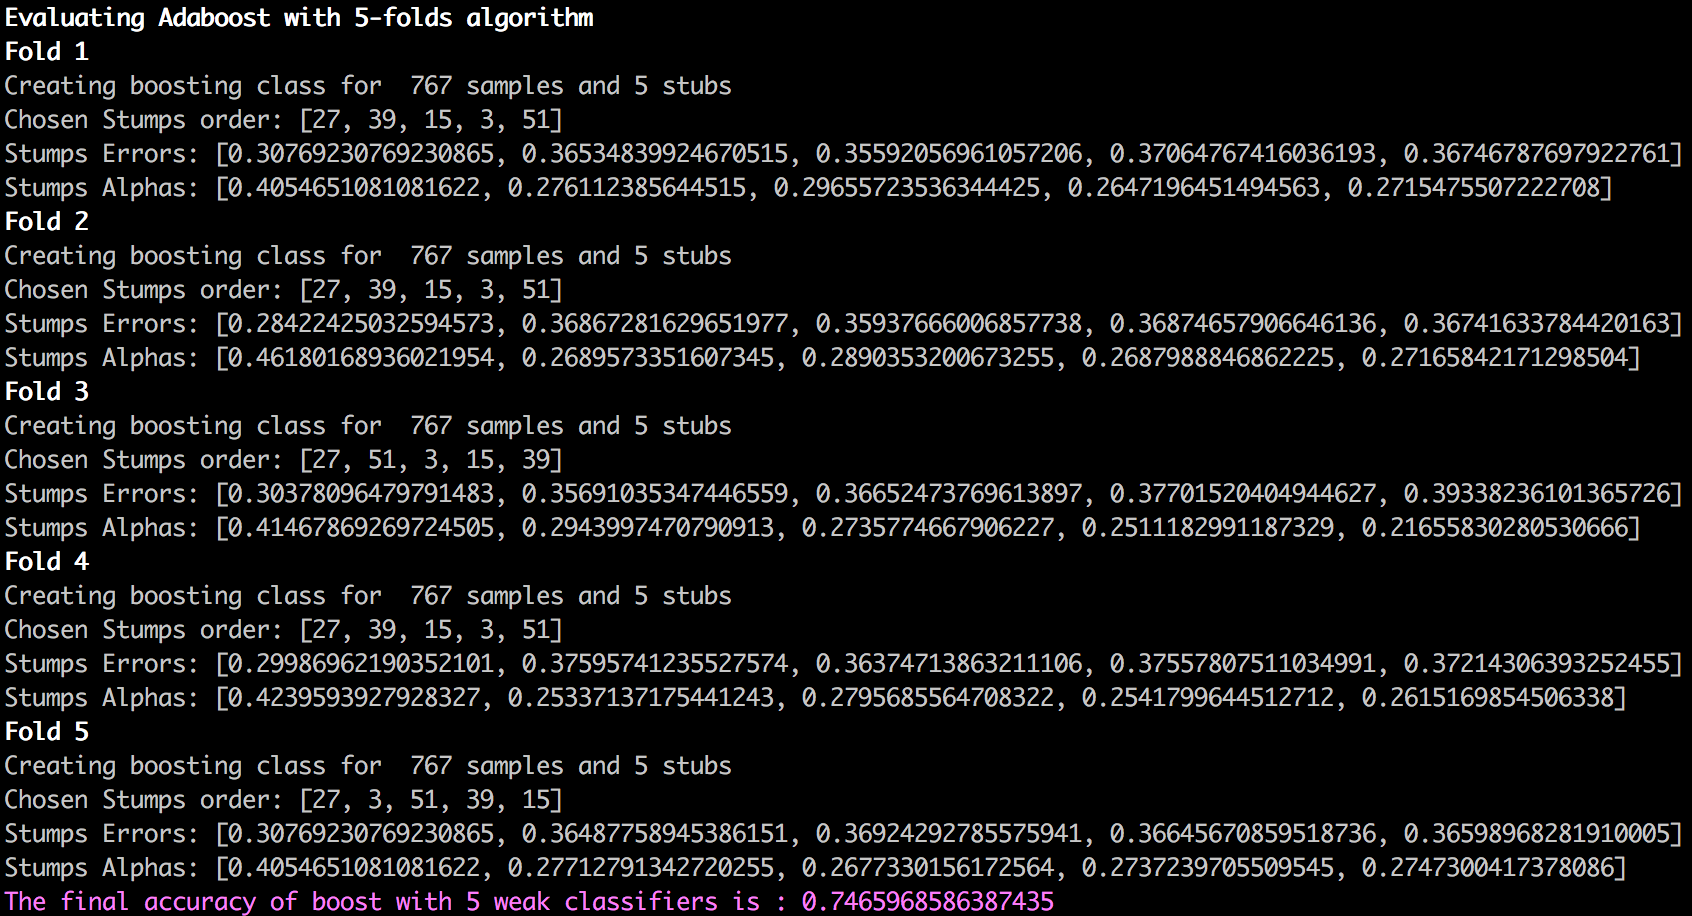
\includegraphics[width=\linewidth]{imgs/exemple_output.png}
  \caption{Resultado da escolha de 5 stumps e 5-fold analise do programa main.py}
	\label{fig:main_5}
\end{figure}


Já o main\_step\_by\_step.py, ele apresentará os resultados parciais de cada escolha de stump, como pode ser visto na Figura.~\ref{fig:main2_2}

\begin{figure}[h!]
  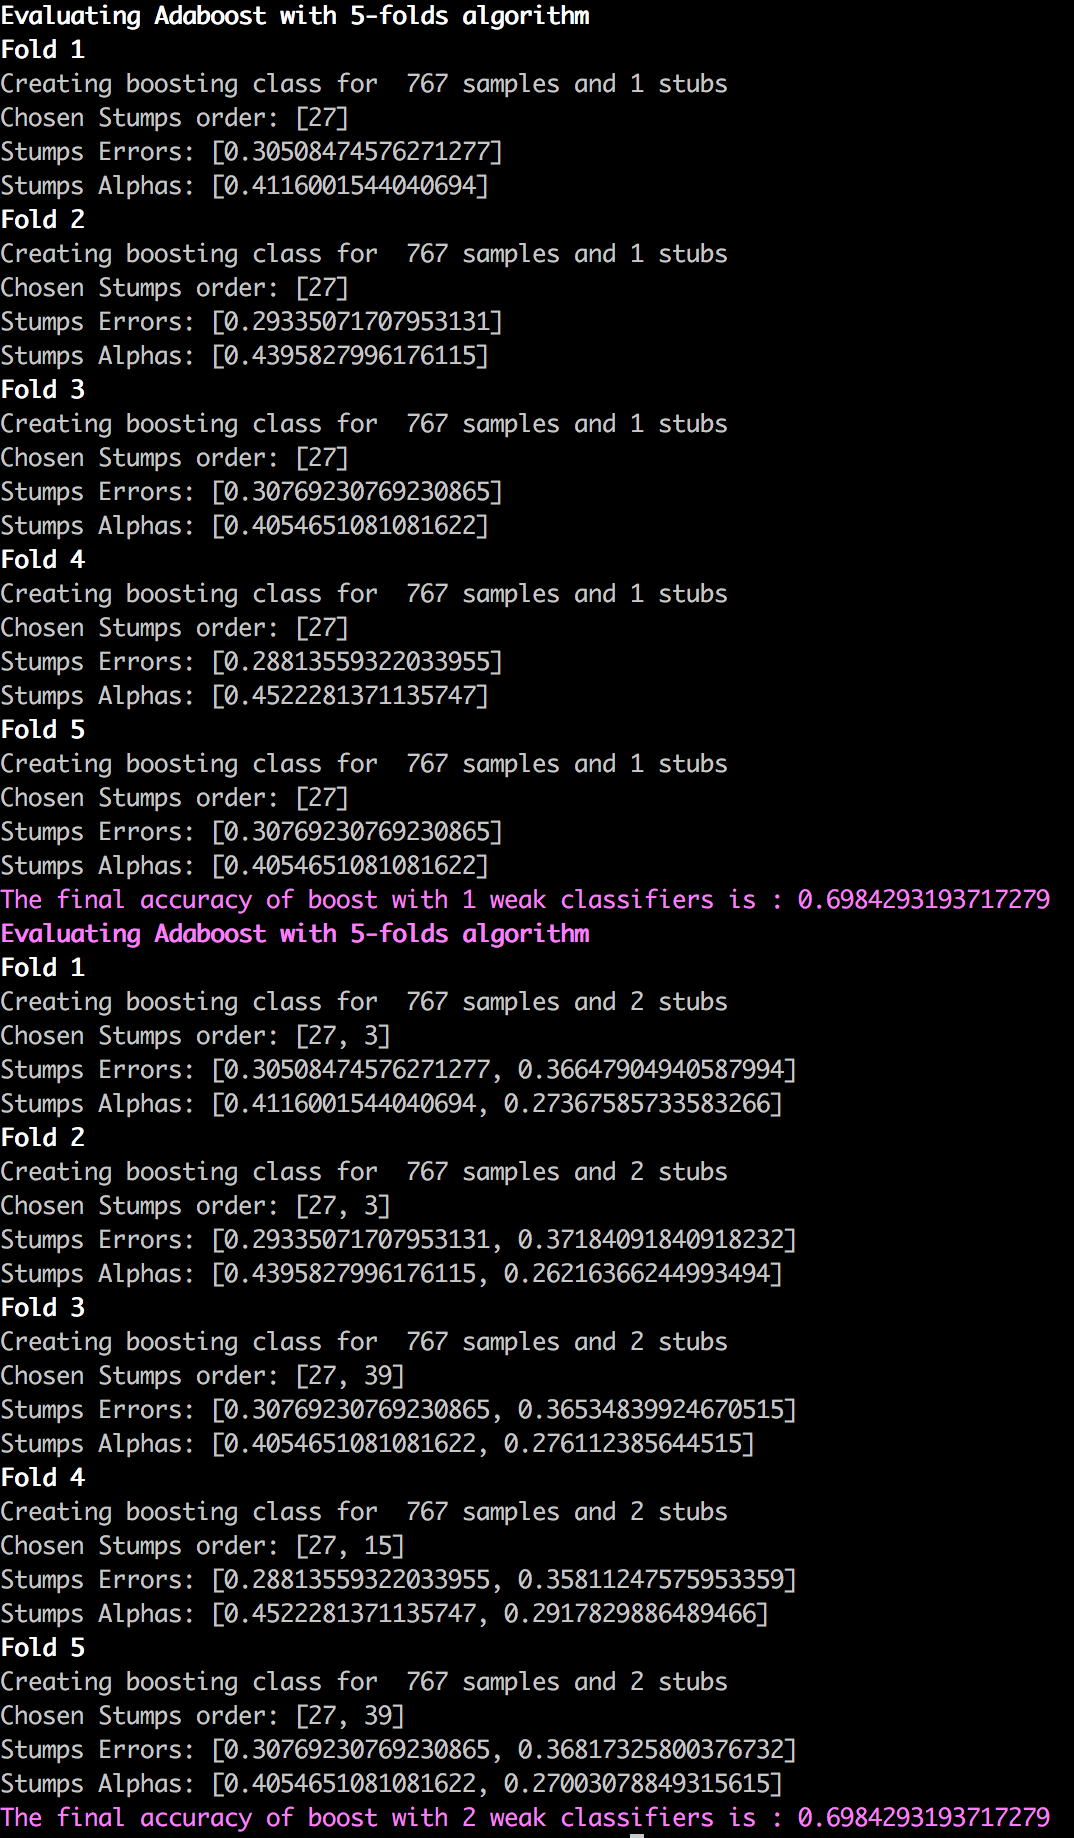
\includegraphics[width=\linewidth]{imgs/exemple_output2.png}
  \caption{Resultado da escolha de 2 stumps e 5-fold analise do programa main\_step\_by\_step.py}
	\label{fig:main2_2}
\end{figure}

Vale a pena atentar para o fato de que os resultados do \emph{Adaboost} com 1 ou 2 stumps são exatamente os mesmos, como mostrado na Figura.~\ref{fig:main2_2}. Este comportamento especifico é esperado pois para cada novo stump escolhido o alpha associado a ele tende a ser menor que o anterior. Logo, no caso de uma combinação de dois classificadores fracos, a classificação sempre será a mesma da da pelo primeiro classificador fraco pois seu alpha é maior que o alpha do segundo, logo a soma do produto da classificação dos dois pelos seus alphas (Algoritimo~\ref{pseudocode:adaboost}, passo 3) sempre terá o sinal do primeiro classificador fraco.


\subsection{Decisões de implementação}
Durante a implementação do algoritmo, algumas decisões importantes foram feitas:

\begin{itemize}
	\item Conforme a especificação original do \emph{Adaboost}, foi permitido que stumps previamente escolhidos pudessem ser escolhidos novamente no futuro.
	\item O base do logaritmo utilizado no calculo dos alphas (Pseudocódigo~\ref{pseudocode:adaboost}) foi a natural $e$
	\item No calculo de novos pesos de cada observação (Pseudocódigo~\ref{pseudocode:adaboost}) a equação original foi expandida e separada em dois casos: quando o stump escolhido acerta e quando ele erra.
\end{itemize}







